\section[IBM]{Immersed Boundary Method}

% Section transition: 05_HYBRID_IMMERSED_BOUNDARY_METHOD
\definecolor{meshGrey}{RGB}{211,211,211}
{\renewcommand{\iceImgX}{1.2}\renewcommand{\iceImgY}{0.50}\renewcommand{\iceImgBg}{meshGrey}%
\IceSectionDivider[height=1.15\H]{}{Immersed\\ Boundary Method}{FIGURES/SECTION_TRANSITION/iceMeshLE_IBM_LAST_LAYER_ADAPTED.png}}


% ---------------------------------------------------------
% Immersed-boundary methods: main approaches
% ---------------------------------------------------------
\begin{frame}{Immersed-Boundary Methods: Main Approaches}

\vspace{0.08cm}

\noindent\resizebox{\textwidth}{!}{Immersed-boundary methods represent solid geometries
without requiring a body-fitted computational mesh.}

\vspace{0.28cm}

\begin{columns}[T,onlytextwidth]

% CUT-CELL
\begin{column}{0.31\textwidth}
\centering
{\color{champsBlue}\bfseries Cut-Cell Method}

\vspace{0.15cm}

\parbox[c][3.0cm][c]{\linewidth}{\centering
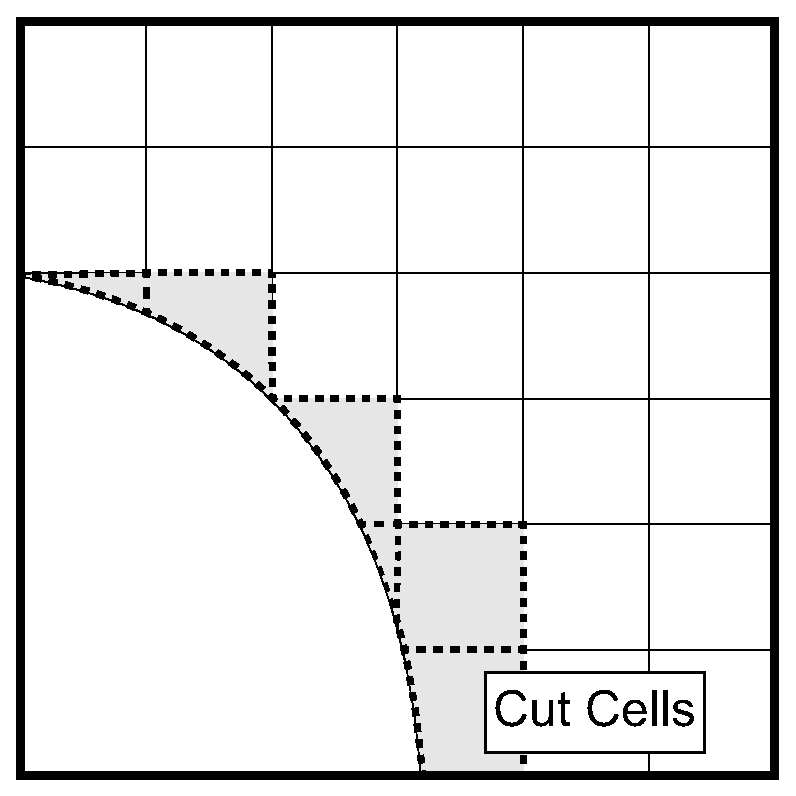
\includegraphics[width=0.96\linewidth,height=2.95cm,keepaspectratio]{FIGURES/IBM/CUT_CELL.eps}
}

\vspace{0.15cm}

\parbox{\linewidth}{\small\raggedright
Modifies intersected control volumes
to conform to the immersed boundary.
}
\end{column}

% PENALIZATION
\begin{column}{0.31\textwidth}
\centering
{\color{champsBlue}\bfseries Penalization Method}

\vspace{0.15cm}

\parbox[c][3.0cm][c]{\linewidth}{\centering
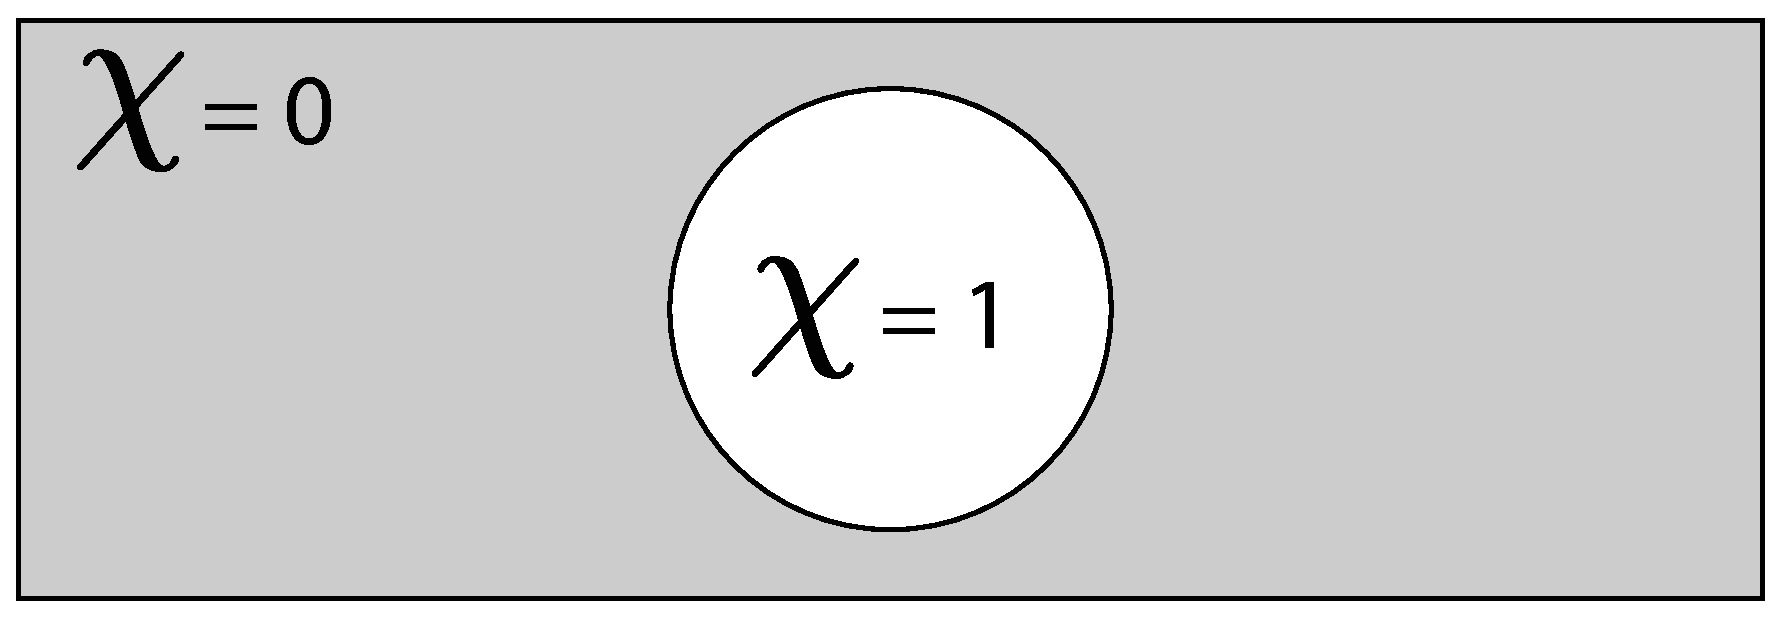
\includegraphics[width=\linewidth,height=2.95cm,keepaspectratio]{FIGURES/IBM/SIMPLIFIED_MASK.eps}
}

\vspace{0.15cm}

\parbox{\linewidth}{\small\raggedright
Introduces source terms to enforce
boundary behavior within the solid region.
}
\end{column}

% GHOST-CELL
\begin{column}{0.31\textwidth}
\centering
{\color{champsBlue}\bfseries Ghost-Cell Method}

\vspace{0.15cm}

\parbox[c][3.0cm][c]{\linewidth}{\centering
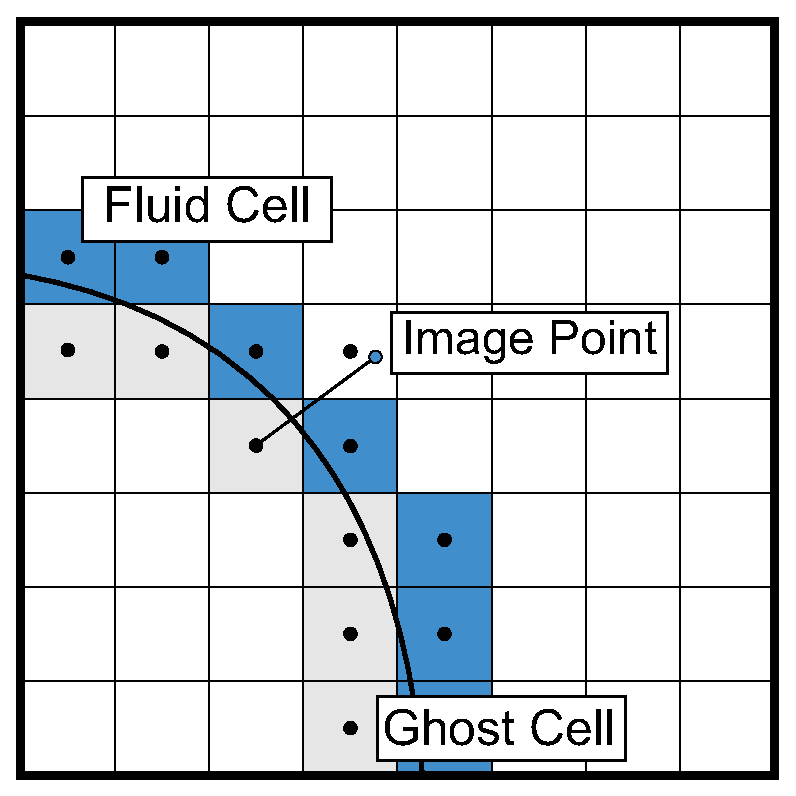
\includegraphics[width=0.96\linewidth,height=2.95cm,keepaspectratio]{FIGURES/IBM/SIMPLIFIED_GC.eps}
}

\vspace{0.15cm}

\parbox{\linewidth}{\small\raggedright
Reconstructs ghost-cell states
to impose immersed-wall boundary conditions.
}
\end{column}

\end{columns}

\vfill

\begin{center}
\begin{tikzpicture}
\node[fill=champsBlue!5, draw=champsBlue!18, rounded corners=4pt,
      text width=0.92\textwidth, inner sep=3pt, align=center, font=\small] {%
\textbf{Existing CHAMPS capability:}
Ghost-cell immersed-boundary RANS solver.};
\end{tikzpicture}
\end{center}

\SlideRef{peskin1972flow,mittal2005immersed,fadlun2000combined,tseng2003ghost,angot1999penalization}
\end{frame}

% 2. EULERIAN IMMERSED DROPLET TREATMENT
\begin{frame}[t]{Eulerian Droplets: Penalization Strategy}
\vspace{-0.15cm}
\small Established penalization strategy integrated into the CHAMPS Eulerian droplet solver.
\par\vspace{0.1cm}
\begin{columns}[T,onlytextwidth]
  \begin{column}{0.32\textwidth}
  \centering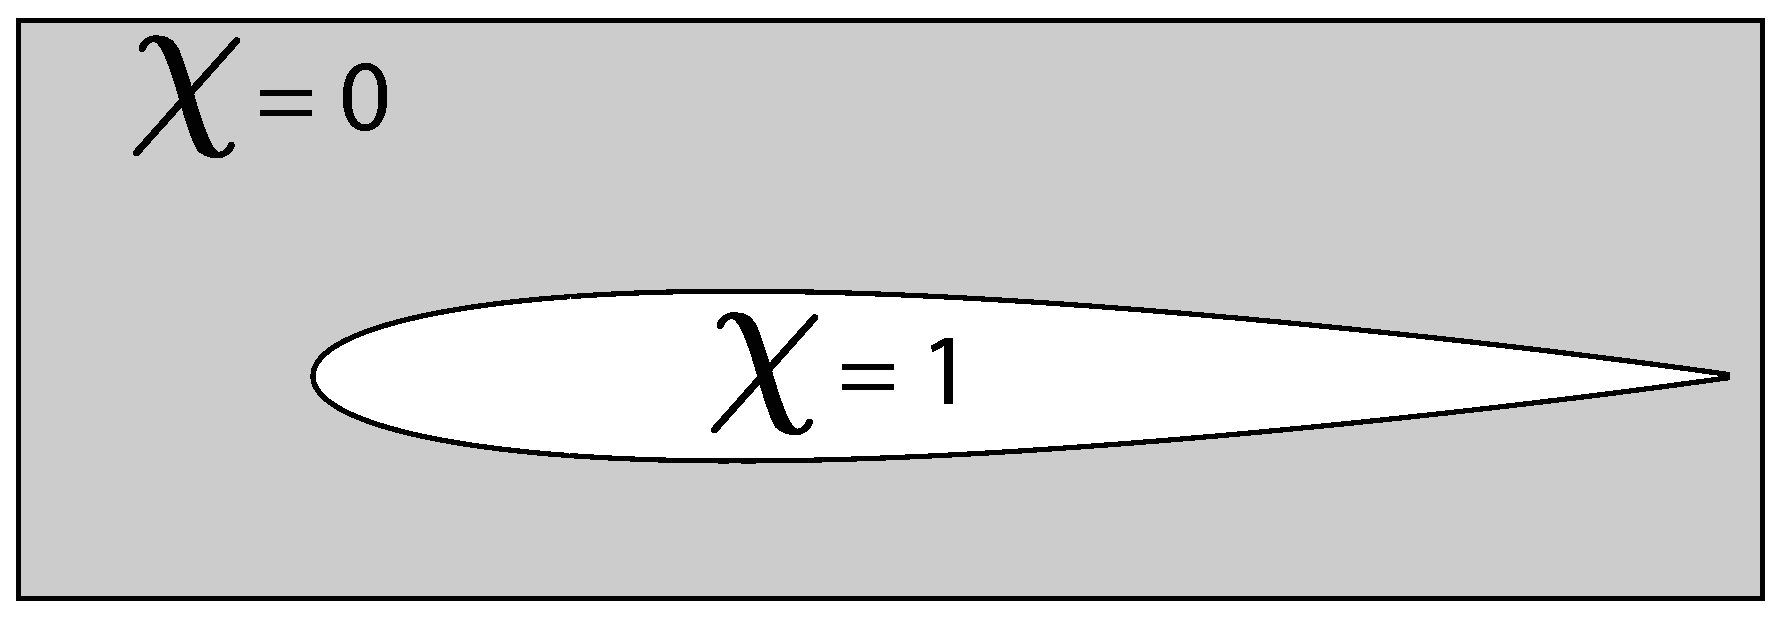
\includegraphics[width=\linewidth,height=1.0cm,keepaspectratio]{FIGURES/IBM/mask}\par
  \vspace{0.02cm}
  {\small\color{champsBlue}\bfseries Solid mask $\chi$}\par
  \end{column}
  \begin{column}{0.32\textwidth}
  \centering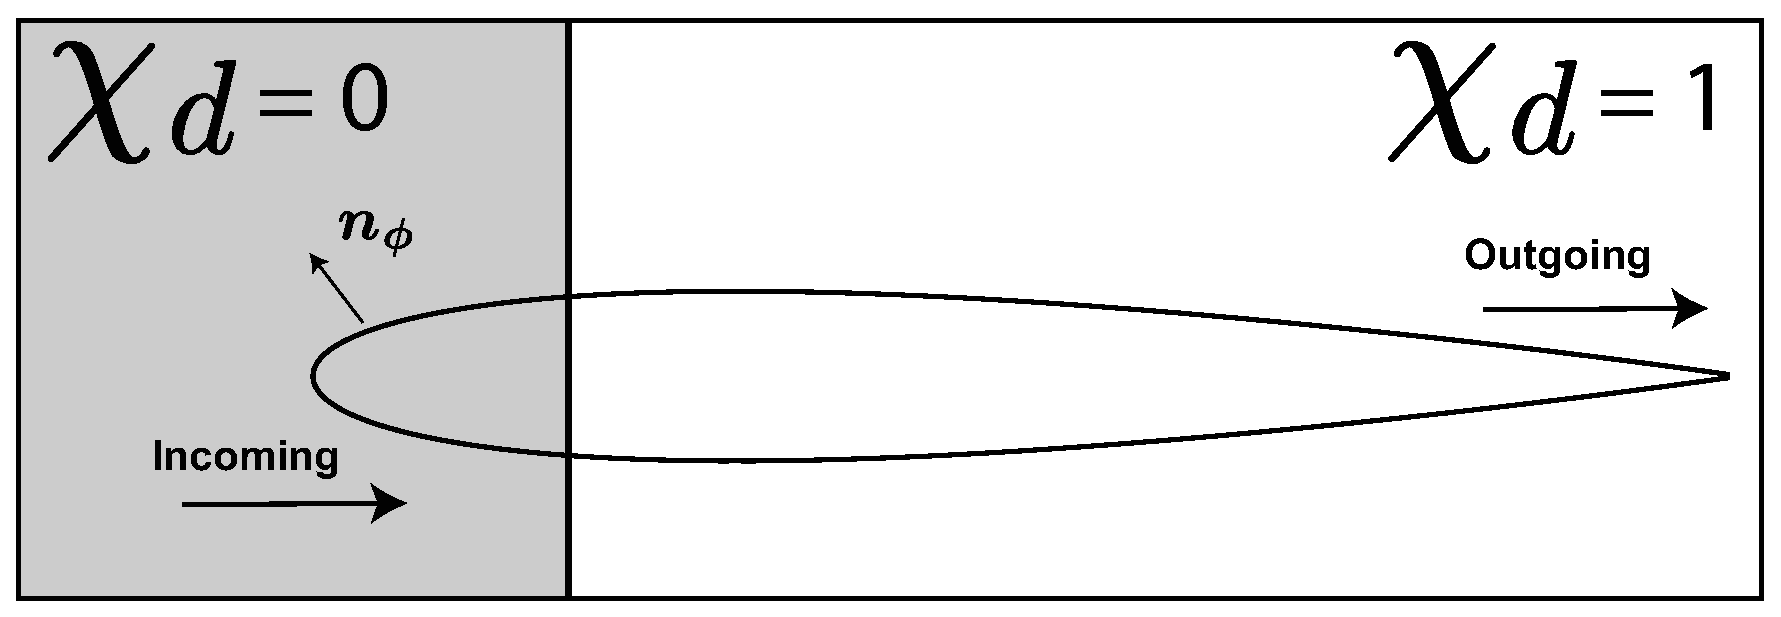
\includegraphics[width=\linewidth,height=1.0cm,keepaspectratio]{FIGURES/IBM/maskChiD}\par
  \vspace{0.02cm}
  {\small\color{champsBlue}\bfseries Direction mask $\chi_d$}\par
  \end{column}
  \begin{column}{0.32\textwidth}
  \centering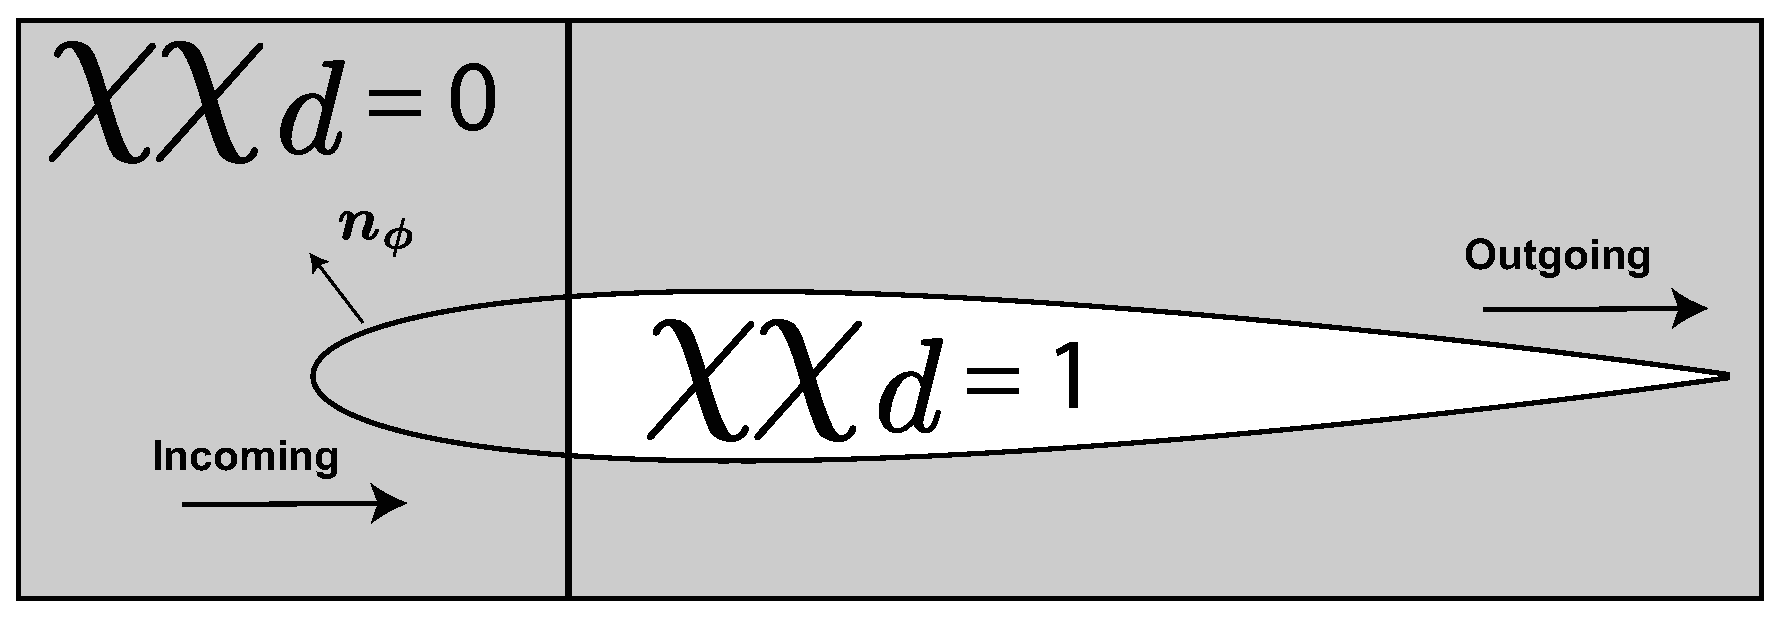
\includegraphics[width=\linewidth,height=1.0cm,keepaspectratio]{FIGURES/IBM/maskChiChiD}\par
  \vspace{0.02cm}
  {\small\color{champsBlue}\bfseries Active mask $\chi\chi_d$}\par
  \end{column}
\end{columns}
\par\vspace*{0.3cm}\mbox{}\par\vspace*{-0.3cm}
\begin{columns}[T,onlytextwidth]
\begin{column}{0.63\textwidth}
{\color{champsBlue}\bfseries Penalized Eulerian Droplet Equations}\par
\vspace{-0.12cm}
{\scriptsize
\begin{align*}
\frac{\partial \alpha}{\partial t}
+\nabla\cdot(\alpha\mathbf{u}_d)
&=
\textcolor{red!80!black}{-}\textcolor{red!80!black}{\underbrace{\frac{\chi\chi_d}{\eta}\alpha}_{\text{Penalization}}}
\\[0.04cm]
\frac{\partial(\alpha\mathbf{u}_d)}{\partial t}
+\nabla\cdot(\alpha\mathbf{u}_d\otimes\mathbf{u}_d)
&=
\textcolor{red!80!black}{(1-\chi)}\left[
\frac{C_DRe_D}{24St}\alpha(\mathbf{u}_a-\mathbf{u}_d)
+\alpha\left(1-\frac{\rho_a}{\rho_d}\right)
\frac{\mathbf{g}}{Fr^2}
\right]
\\
&\quad\textcolor{red!80!black}{-}
\textcolor{red!80!black}{\underbrace{\frac{\chi\chi_d}{\eta}\alpha\mathbf{u}_d}_{\text{Penalization}}}
\end{align*}}
\end{column}
\hfill
\begin{column}{0.34\textwidth}
{\color{champsBlue}\bfseries Direction Mask}\par
\vspace{0.04cm}
{\centering\scriptsize$\chi_d=\begin{cases}1, & \mathbf{u}_d\cdot\mathbf{n}_{\phi}\leq 0,\\ 0, & \mathbf{u}_d\cdot\mathbf{n}_{\phi}>0.\end{cases}$\par}
\vspace{0.1cm}
{\color{champsBlue}\bfseries Main Benefits}\par
\vspace{0.02cm}
\begin{itemize}\footnotesize\setlength{\itemsep}{1pt}
  \item Limited solver modifications.
  \item Body-fitted-like impingement predictions.
  \item Second-order spatial convergence recovered in verification.
\end{itemize}
\end{column}
\end{columns}
\vfill
\begin{center}
\begin{tikzpicture}
\node[fill=champsBlue!5, draw=champsBlue!18, rounded corners=4pt,
      text width=\textwidth-0.2cm, inner sep=3pt, align=center, font=\small] {%
\textbf{Penalization acts only in the incoming-droplet region inside the immersed body.}};
\end{tikzpicture}
\end{center}
\SlideRef{angot1999penalization,lavoieDroplets}
\end{frame}

% 3. LAGRANGIAN IMMERSED-SURFACE IMPACT DETECTION
\begin{frame}{Lagrangian Droplets: Immersed-Surface Impacts}
\vspace{0.06cm}
\begin{columns}[c,onlytextwidth]
\begin{column}{0.42\textwidth}
{\color{champsBlue}\bfseries Preserve Face-to-Face Tracking}\par
\vspace{0.10cm}
\begin{itemize}\setlength{\itemsep}{4pt}
  \item Advance trajectories through the \textbf{background volume mesh}.
  \item Pre-tag cells cut by the immersed surface.
  \item On entry, test the trajectory ray against associated surface facets.
  \item \textbf{Axis-Aligned Bounding Box (AABB) tree geometry queries} accelerate closest-point and intersection operations.
\end{itemize}
\vspace{0.15cm}
{\small\color{champsBlue}\bfseries Everything else is kept from the body-fitted solver; only the impact-position detection changes.\par}
\end{column}
\hfill
\begin{column}{0.55\textwidth}
\centering
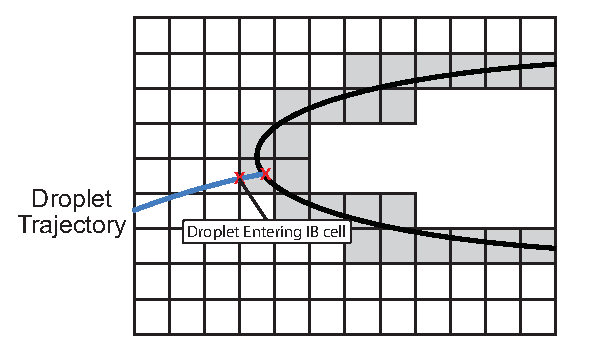
\includegraphics[width=\linewidth,height=5.0cm,keepaspectratio]{FIGURES/IBM/surfaceIntersection}\par
\vspace{0.06cm}
{\scriptsize\color{gray}Intersection of the droplet trajectory with the immersed surface.}
\end{column}
\end{columns}
\SlideRef{pabloThesis}
\end{frame}

% 4. IBM LEVEL-SET COUPLING
\begin{frame}[t]{IBM--Level-Set Icing Framework}
\vspace{0.04cm}
\small The \textbf{aerodynamic and droplet} fields use a nonconformal IBM background mesh;
\textbf{geometry evolution} retains an adapted, body-fitted auxiliary mesh.
\vspace{0.22cm}
\begin{center}
\begin{tikzpicture}[>=stealth,
    every node/.style={align=center,font=\scriptsize,execute at begin node={\hyphenpenalty=10000}},
    stage/.style={draw=champsBlue!35,fill=champsBlue!7,rounded corners=3pt,
       minimum height=1.08cm,text width=3.25cm,inner sep=3pt}]
  \node[stage] (flow) at (0,0) {\textbf{RANS + Droplets}\\IBM background mesh};
  \node[stage] (thermo) at (3.65,0) {\textbf{Thermodynamics}\\Conformal ice surface};
  \node[stage] (ls) at (7.30,0) {\textbf{Level Set}\\Adapted auxiliary mesh};
  \node[stage] (geom) at (10.95,0) {\textbf{Ice Extraction}\\Updated immersed surface};
  \draw[->,line width=0.8pt,champsBlue] (flow)--(thermo);
  \draw[->,line width=0.8pt,champsBlue] (thermo)--(ls);
  \draw[->,line width=0.8pt,champsBlue] (ls)--(geom);
  \draw[->,line width=0.9pt,champsBlue] (geom.south) -- ++(0,-0.65) -| (flow.south);
  \node[fill=white,text=champsBlue,font=\scriptsize] at (5.475,-1.70)
  {Update signed distance and masks; recompute next layer};
\end{tikzpicture}
\end{center}
\vspace{0.16cm}
\begin{columns}[T,onlytextwidth]
\begin{column}{0.48\textwidth}
{\color{champsBlue}\bfseries Why Keep the Level-Set Mesh Body-Fitted?}\par
\vspace{0.10cm}
\small The auxiliary level-set mesh is easier to adapt than a RANS
mesh, since no thin boundary-layer cells are required.
\end{column}
\hfill
\begin{column}{0.48\textwidth}
{\color{champsBlue}\bfseries Preserve the Clean Geometry}\par
\vspace{0.10cm}
\small Restrict evolution and reconstruction to the ice-growth region;
retain unaffected geometry rather than moving the full interface.
\end{column}
\end{columns}
\vfill
\begin{center}
\begin{tikzpicture}
\node[fill=champsBlue!5, draw=champsBlue!18, rounded corners=4pt,
      text width=0.92\textwidth, inner sep=3pt, align=center, font=\small] {%
\textbf{Avoid repeated body-fitted RANS remeshing, not all auxiliary meshing.}};
\end{tikzpicture}
\end{center}
\SlideRef{lavoieLevelSet,lavoie2021immersed,pabloThesis}
\end{frame}

% 5. SLD NACA 23012
\begin{frame}[t]{IBM Impingement Results: NACA 23012 (SLD)}
\vspace{-0.3cm}
\begin{center}
{\scriptsize\color{champsBlue}\bfseries NACA 23012 \quad
$\bm{M_\infty=0.232}$ \quad \textbf{AoA} $\bm{=2.5^\circ}$ \quad
LWC $=0.50$ g/m$^3$ \quad MVD $=111\,\mu$m}
\end{center}
\vspace{0.06cm}
\begin{columns}[T,onlytextwidth]
  \begin{column}{0.49\textwidth}
    \centering
    {\color{champsBlue}\bfseries Eulerian}\par\vspace{0.08cm}
    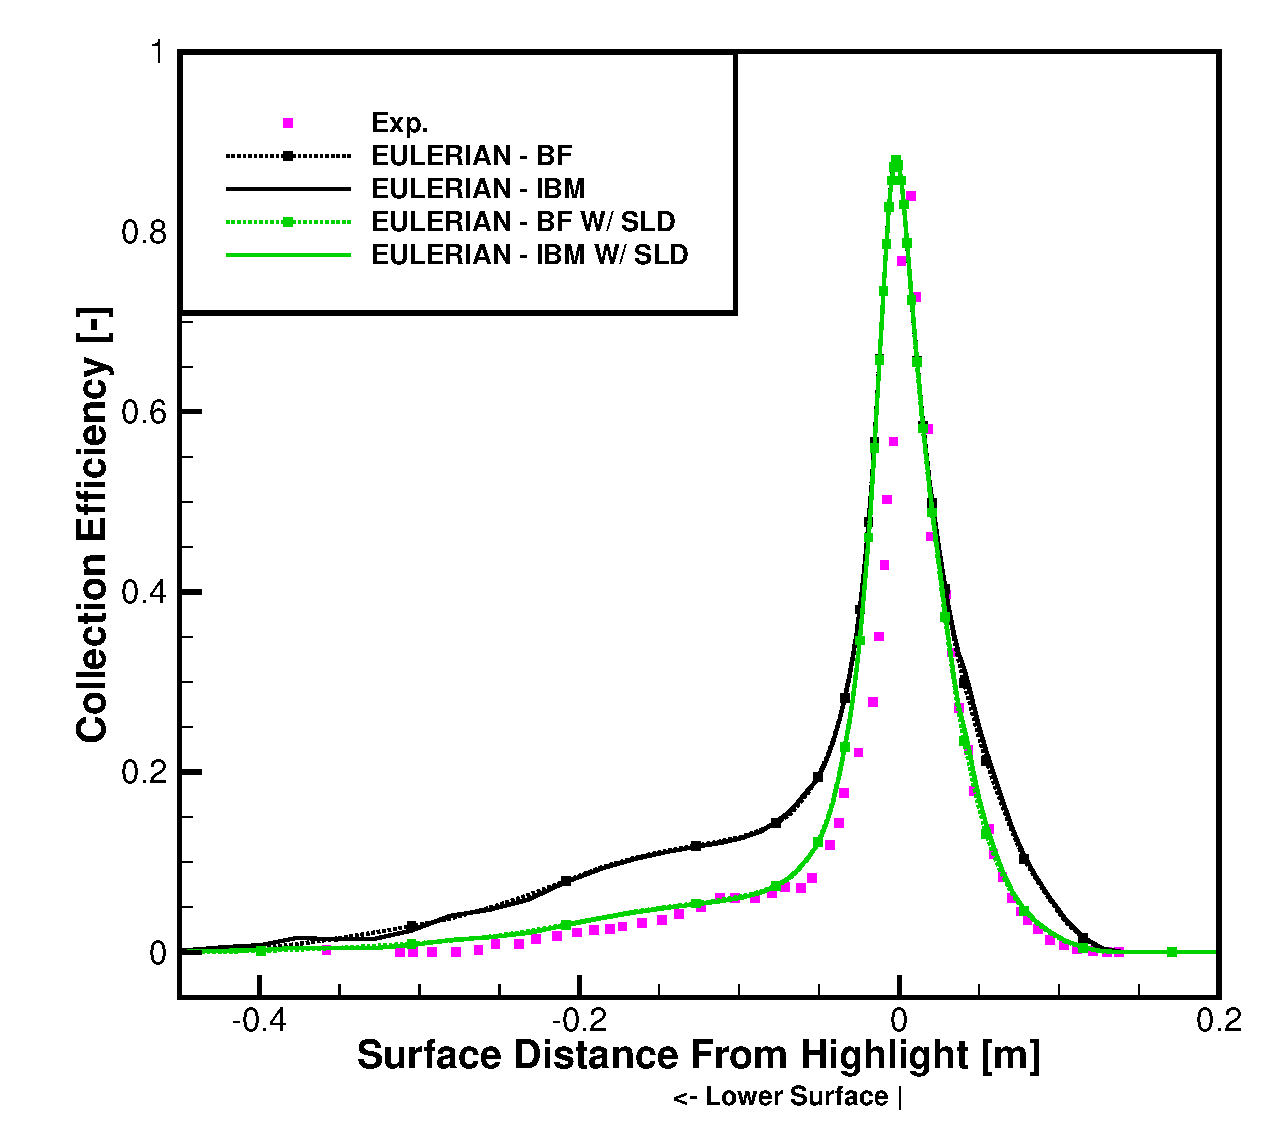
\includegraphics[width=\linewidth,height=4.95cm,keepaspectratio]{FIGURES/IBM/CASE_SLD_EULERIAN_BETA}
  \end{column}
  \hfill
  \begin{column}{0.49\textwidth}
    \centering
    {\color{champsBlue}\bfseries Lagrangian}\par\vspace{0.08cm}
    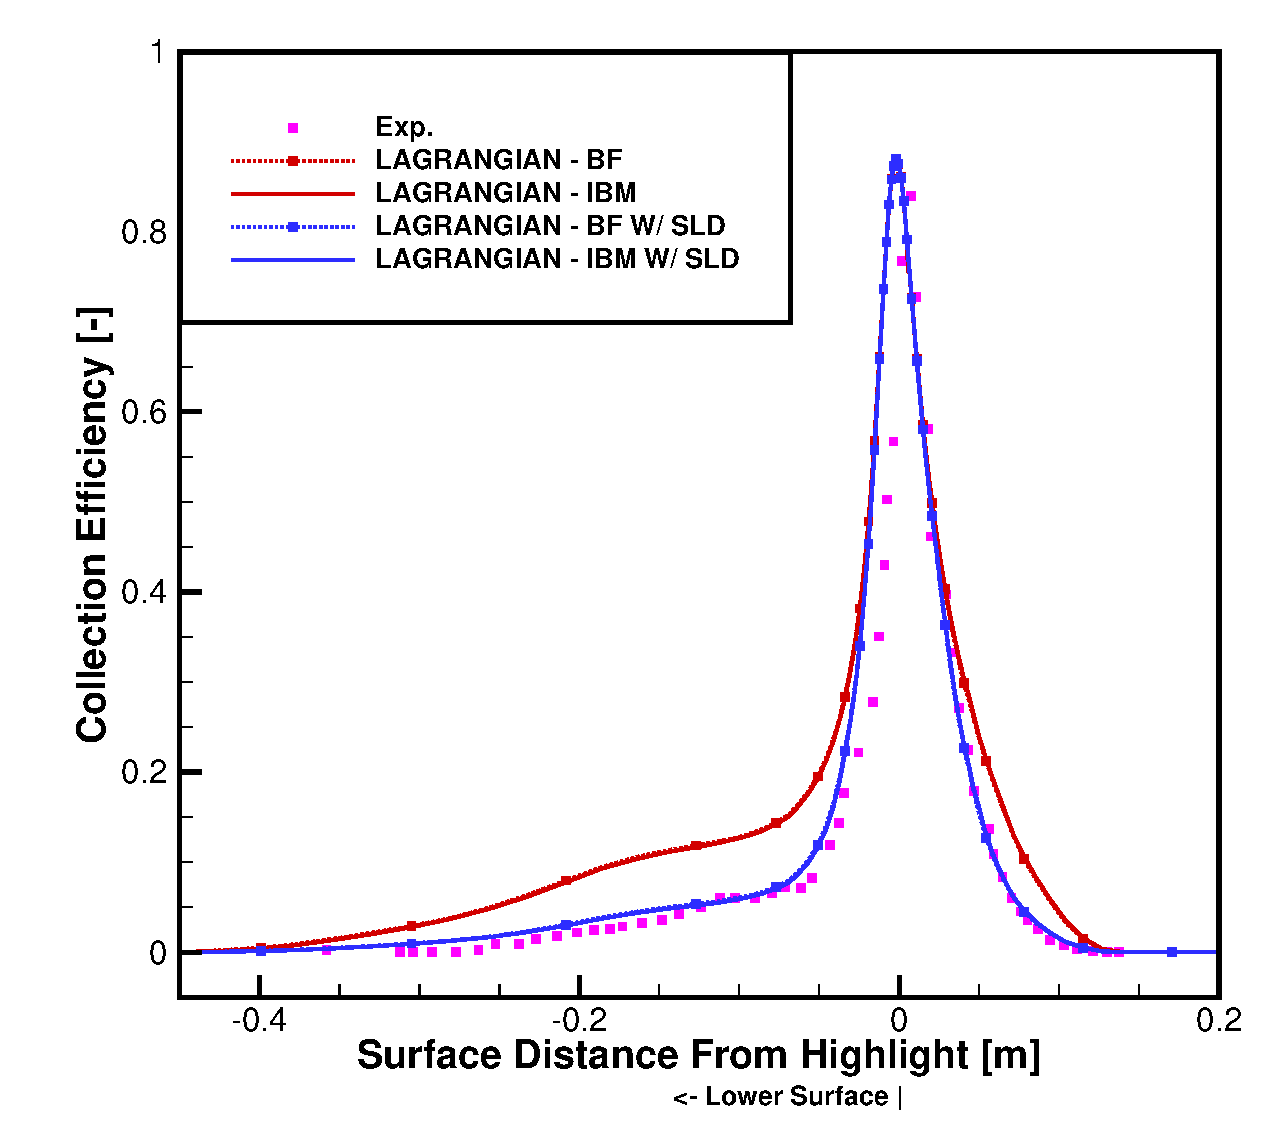
\includegraphics[width=\linewidth,height=4.95cm,keepaspectratio]{FIGURES/IBM/CASE_SLD_LAGRANGIAN_BETA}
  \end{column}
\end{columns}
\vspace{-0.15cm}
\begin{center}
\begin{tikzpicture}
\node[fill=champsBlue!5, draw=champsBlue!18, rounded corners=4pt,
      text width=0.92\textwidth, inner sep=3pt, align=center, font=\small] {%
\textbf{BF and IBM agree closely} for both droplet formulations;
SLD splashing corrections improve experimental agreement.};
\end{tikzpicture}
\end{center}
\SlideRef{papadakis2007large}
\end{frame}

% 6. NACA0012 RIME
\begin{frame}[t]{IBM Ice Accretion Results: Rime (Case 01)}
\vspace{0.06cm}
\begin{center}
{\scriptsize\color{champsBlue}\bfseries NACA 0012 \quad
$\bm{M_\infty=0.325}$ \quad \textbf{AoA} $\bm{=4^\circ}$ \quad
LWC $=0.60$ g/m$^3$ \quad MVD $=20\,\mu$m \quad Exposure time $=420$ s}
\end{center}
\vspace{-0.15cm}
\begin{columns}[c,onlytextwidth]
\begin{column}{0.61\textwidth}
\centering
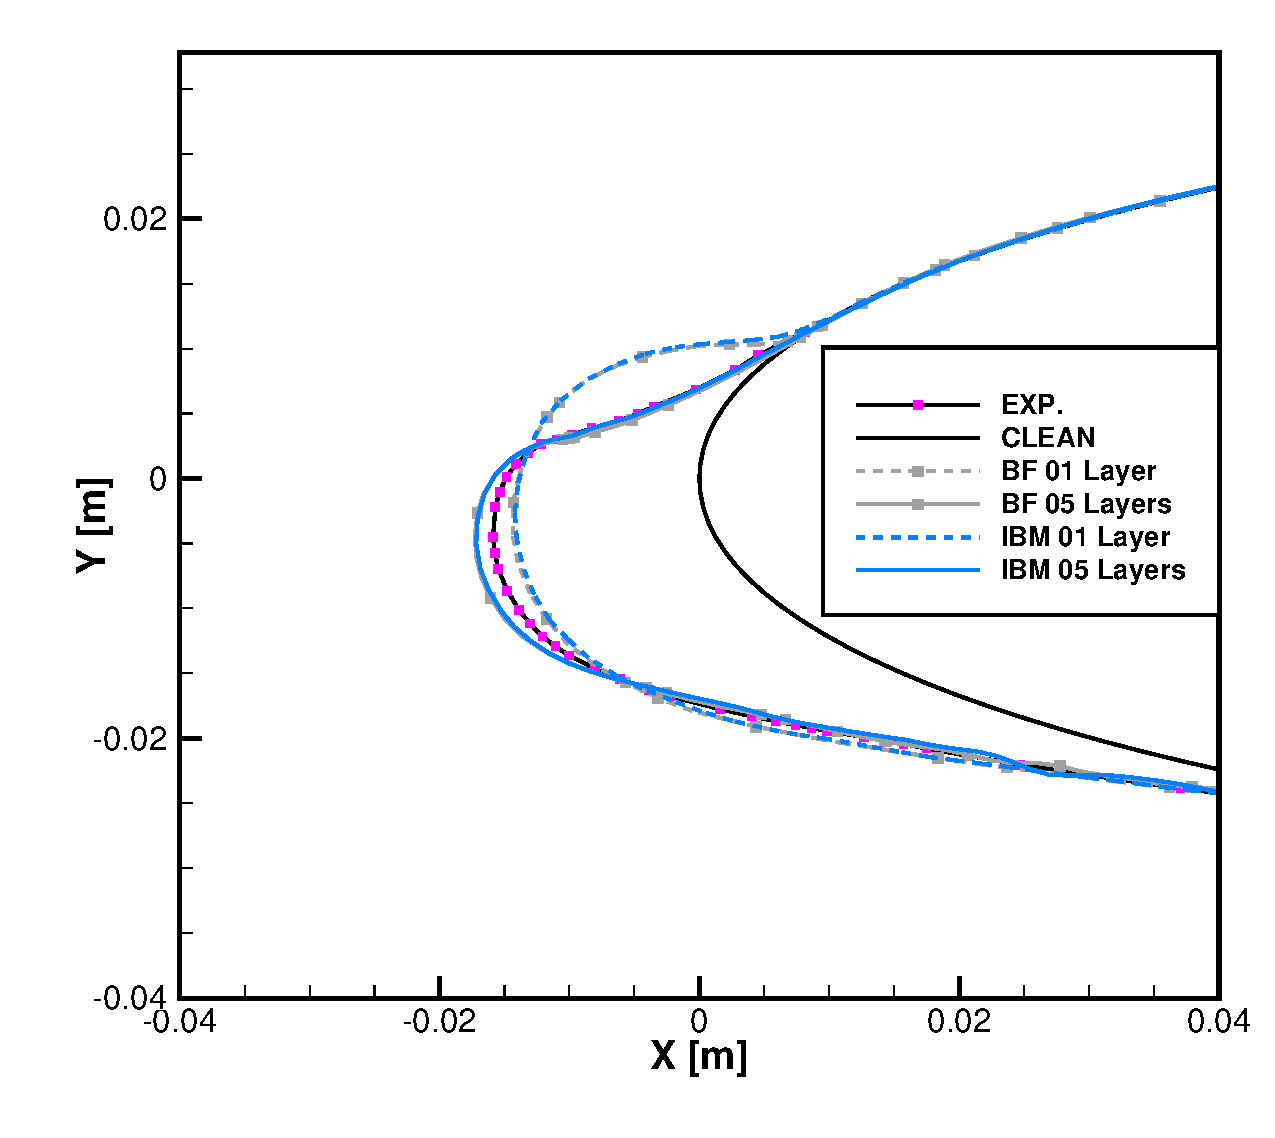
\includegraphics[width=\linewidth,height=5.3cm,keepaspectratio]{FIGURES/IBM/CASE_01_ICE_SHAPE}
\end{column}
\hfill
\begin{column}{0.36\textwidth}
{\color{champsBlue}\bfseries Main Observations}\par
\vspace{0.08cm}
\begin{itemize}\setlength{\itemsep}{5pt}
  \item Close \textbf{BF--IBM agreement}.
  \item Good agreement with experiments.
  \item Five-layer prediction improves over single-step.
\end{itemize}
\end{column}
\end{columns}
\vfill
\begin{center}
\begin{tikzpicture}
\node[fill=champsBlue!5, draw=champsBlue!18, rounded corners=4pt,
      text width=0.92\textwidth, inner sep=3pt, align=center, font=\small] {%
\textbf{Impingement-driven ice accretion (rime cases) is very well predicted with the IBM.}};
\end{tikzpicture}
\end{center}
\end{frame}

% 7. NACA0012 GLAZE / HTC
\begin{frame}[t]{IBM Ice Accretion Results: Glaze (Case 04)}
\vspace{-0.3cm}
\begin{center}
{\scriptsize\color{champsBlue}\bfseries NACA 0012 \quad
$\bm{M_\infty=0.317}$ \quad \textbf{AoA} $\bm{=4^\circ}$ \quad
LWC $=0.55$ g/m$^3$ \quad MVD $=15\,\mu$m \quad Exposure time $=384$ s}
\end{center}
\vspace{-0.1cm}
\begin{columns}[T,onlytextwidth]
  \begin{column}{0.495\textwidth}
    \centering {\color{champsBlue}\bfseries Five-Layer Ice Shape}\par\vspace{0.06cm}
    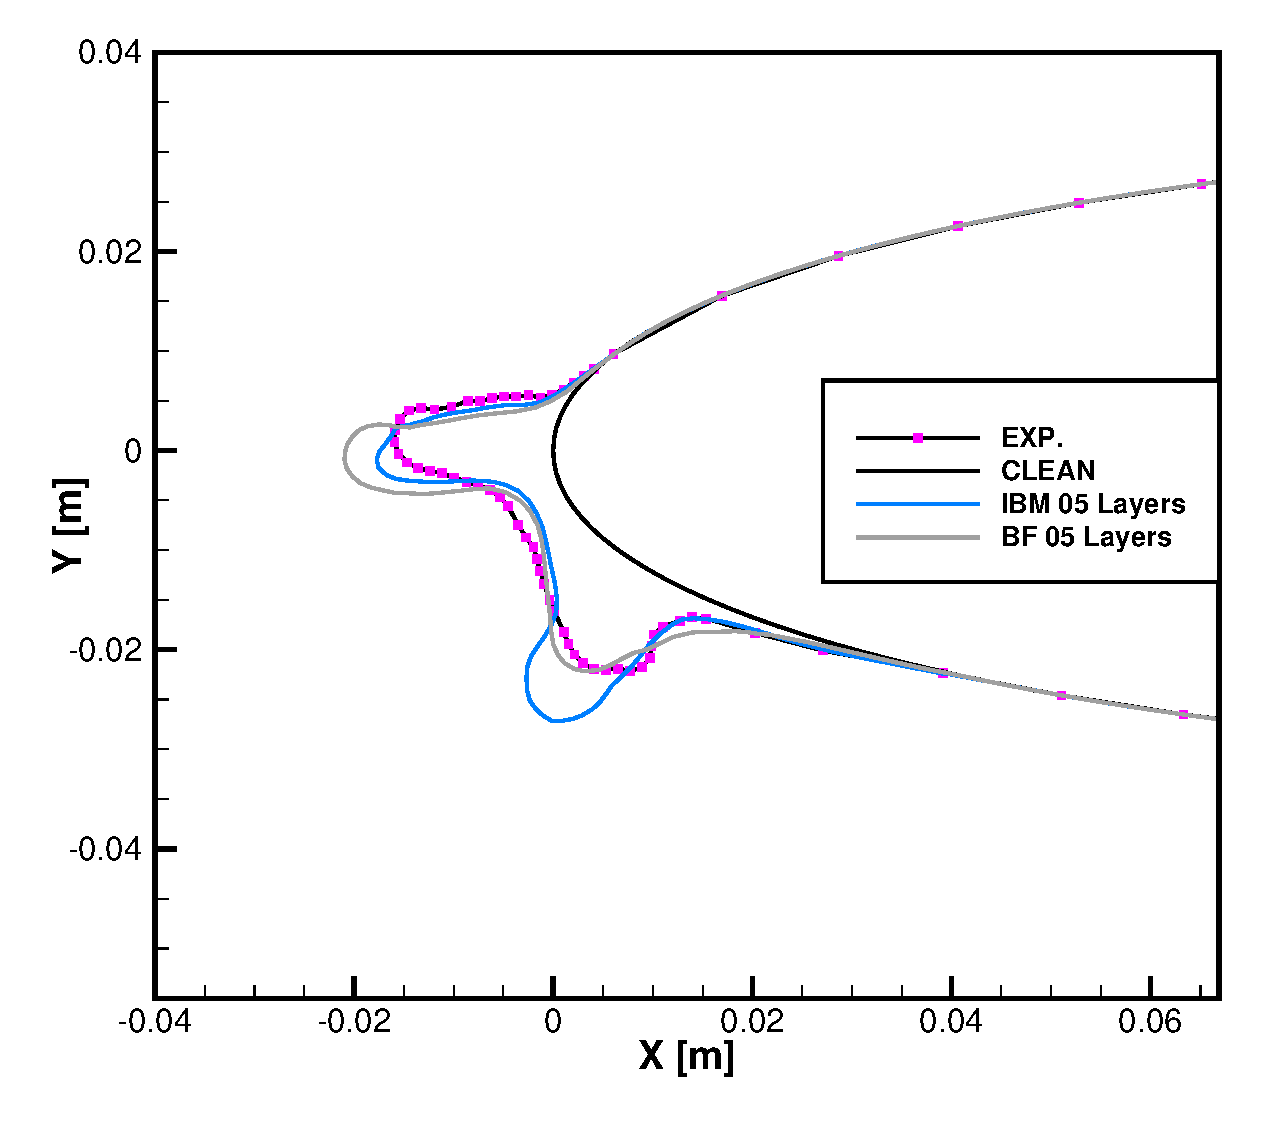
\includegraphics[width=\linewidth,height=5.45cm,keepaspectratio]{FIGURES/IBM/CASE_04_ICE_SHAPE_05_LAYER}
  \end{column}
  \hfill
  \begin{column}{0.495\textwidth}
    \centering {\color{champsBlue}\bfseries Convective Heat Transfer}\par\vspace{0.06cm}
    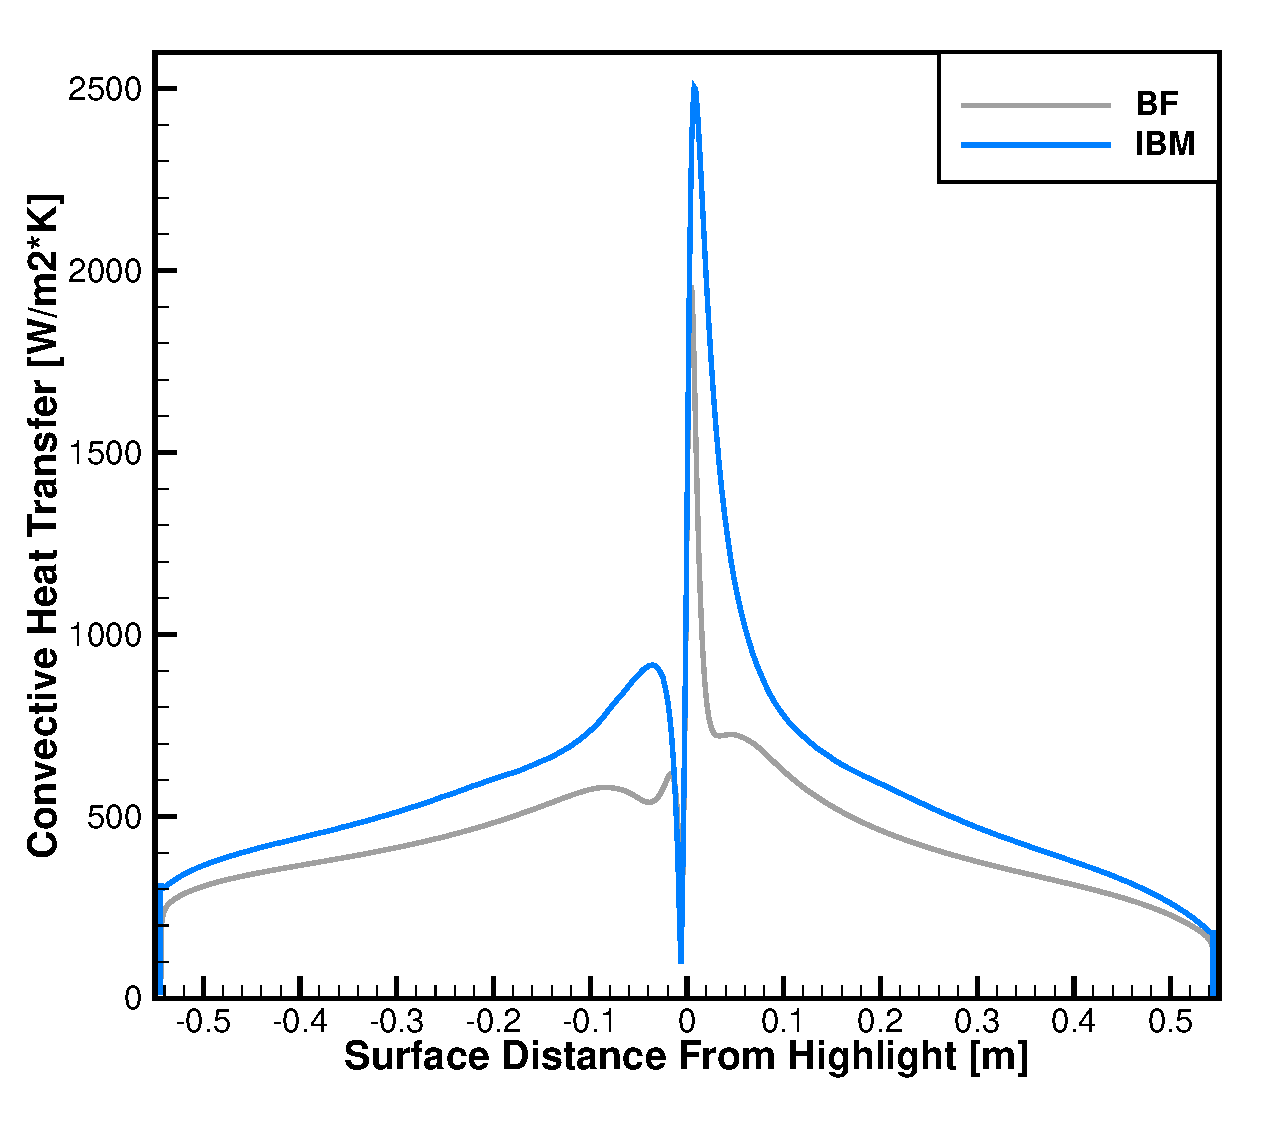
\includegraphics[width=\linewidth,height=5.45cm,keepaspectratio]{FIGURES/IBM/CASE_04_HTC}
  \end{column}
\end{columns}
\vspace{-0.2cm}
\begin{center}
\begin{tikzpicture}
\node[fill=champsBlue!5, draw=champsBlue!18, rounded corners=4pt,
      minimum width=0.98\textwidth, inner sep=3pt, font=\footnotesize] {%
Both reproduce glaze horns, but \textbf{near-wall HTC differences} accumulate across layers, especially around the lower horn.};
\end{tikzpicture}
\end{center}
\end{frame}

